\selectlanguage{english}
\begin{abstract}
    \noindent A \emph{Számítógépes szimulációk} című laboratúrium első alkalmával az egyszerű, 1 dimenziós harmonikus oszcillátor numerikus megoldását járjuk körül, mely a félévi tárgy bevezetőjeként szolgál. A szimuláció forráskódja C++ nyelven, az ábrák pedig egy Jupyter Notebook-ban futó Python 3 kernel alatt készültek. A beadandó első célja a forráskóddal történő ismerkedés, valamint a paraméterek változtatásával történő különböző kezdőfeltételek beállítása és a szimuláció futtatása volt. Ezt követően az ebből kapott különböző kimenetek, megadott szempontok alapján történő elemzése volt a feladatunk. \\
\end{abstract}
\selectlanguage{magyar}

\begin{multicols}{2}
\section{Bevezetés és elmélet} \label{sec:1}
A Számítógépes szimulációk laboratórium első feladata során az egyszerű 1-dimenziós, harmonikus oszcillátor mozgását vizsgáltuk. Fizikai modelljének leírása és a szimuláció forráskódja már előzetesen a rendelkezésünkre állt a tárgy honlapján\cite{szamszin}. \\
Az 1D harmonikus oszcillátort az alábbi mozgásegyenlettel írhatjuk le:

\begin{equation} \label{eq:1.1}
    m * \ddot{x} \left( t \right)  = - m * \omega^{2} * x \left( t \right)
\end{equation}
Ennek a differenciálegyenletnek az analitikus megoldását egy megfelelő Ansatz segítségével kaphatjuk meg a legkönnyebben. Az egyenlet megoldása a következő lesz:

\begin{equation} \label{eq:1.2}
    x \left( t \right)  = x_{0} * \cos(\omega t) + \frac{v_{0}}{\omega} * \sin(\omega t)
\end{equation}
A numerikus megoldáshoz a mozgásegyenlet alábbi formáját használjuk fel:

\begin{equation} \label{eq:1.3}
    \frac{d^{2} x \left( t \right) }{d t^{2}} = - \omega^{2} x \left( t \right) 
\end{equation}
Ugyanis ezt felbonthatjuk a következő két, elsőrendő, csatolt egyenletre:

\begin{equation} \label{eq:1.4}
    \frac{dx \left( t \right)}{dt} = v \left( t \right) 
\end{equation}

\begin{equation} \label{eq:1.5}
    \frac{dv \left( t \right)}{dt} = - \omega^{2} * x \left( t \right) = a \left( t \right)
\end{equation}
Ez az egyenletrendszer analitikusan is könnyen megoldható, azonban a gyakorlás kedvéért numerikus megoldáshoz folyamodunk.

\section{Feladatok} \label{sec:2}
Az első szimuláció során négy darab feladatot volt szükséges teljesíteni a rendelkezésre álló forráskód fordítása után. \\
Az első a harmonikus oszcillátor kitérés-idő diagramjának felvétele tetszőlegesen hosszú időtartamra. \\
A második feladatban az oszcillátor kitérés-sebesség diagramját kell vizsgálnunk hosszú időtartamra. Itt elemeznünk és diszkutálnunk is kell a kapott eredményt, hogy miben tér el a várt képtől. \\
A harmadik feladat az Euler-Cromer és a szimpla Euler differenciálegyenlet megoldási módszerek összehasonlítása az energiamegmaradás szempontjából. A fő kérdés, hogy melyiknél és hogyan marad, vagy nem marad meg az energia? \\
A negyedik feladat során a szimuláció futásidejét kell tesztelnünk és megvizsgálnunk a megoldási módszerekben használt lépésszám függvényében.

\section{Megvalósítás} \label{sec:3}
A szimuláció forráskódja C++ nyelven készült és az Euler-Cromer megoldási módszert alkalmazza, mely az Euler módszer apró bővítéssel ellátott verziója. Az Euler módszer lényege a következő, a fent ismertetett egyenleteken keresztül bemutatva\cite{csabaidiff}:

\begin{equation}
    x \left(t + \Delta t \right) = x \left( t \right) + v \left( t \right) * \Delta t
\end{equation}

\begin{equation}
    v \left(t + \Delta t \right) = v \left( t \right) + x \left( t \right) * \Delta t
\end{equation}

\begin{equation}
    t \to t + \Delta t
\end{equation}
Ennek módosított variációja a már említett Euler-Cromer módszer, ahol a második lépésben nem a $t$, hanem a $t + \Delta t$ helyen levő értékkel történik a kiértékelés. A módszer kontraintuitívnak tűnhet az alábbi módon:

\begin{equation}
    x \left(t + \Delta t \right) = x \left( t \right) + v \left( t \right) * \Delta t
\end{equation}

\begin{equation}
    v \left(t + \Delta t \right) = v \left( t \right) + x \left( t + \Delta \right) * \Delta t
\end{equation}

\begin{equation}
    t \to t + \Delta t
\end{equation}
Mindkét esetben az $x \left( t = 0 \right)$ és a $v \left( t = 0 \right)$ értékekkel inicializáljuk a szimulációnkat, majd addig futtatjuk, míg a $t$ érték el nem ér egy tetszőleges $t_{max}$ felső korlátot. $\Delta t$ a szimuláció lépésközét jelöli, amit szintén mi választunk meg. \\
Várakozásaink szerint az utóbbi módszer előnye, hogy szinte megtartja az energiát, míg az első nem\cite{cromer}. Ez persze egyéb módszerek segítségével még tovább javítható\cite{Iserles-2003}. Ennek vizsgálata majd a harmadik részfeladatban fog megtörténni.

\subsection{A rendelkezésre álló kód modosításai}
A forráskódot egy segéd batch file segítségével fordítottam le, abban clang fordítót használva, mely kimeneti binárisa így egy \code{sho.exe} lett. Az \cite{szamszin} linken elérhető forráskód ellenben apró módosításokra szorult. Ezek a módosítások elsősorban azt eredményezték, hogy a szimuláció végleges kimenetként egy \emph{sho.dat} nevű file-t generál, ami az adatokat az \ref{tab1}. táblázatnak megfelelő elrendezésben tartalmazza:

\begin{center}
\begin{tabular}{c|c|c|c}
$t$ & $x \left( t \right)$ & $v \left( t \right)$ & $E \left( t \right)$ \\
\hline \hline
$0$ & $x \left( 0 \right)$ & $v \left( 0 \right)$  & $E \left( 0 \right)$ \\
\hline
$\Delta t$ & $x \left( \Delta t \right)$ & $v \left( \Delta t \right)$ & $E \left( \Delta t \right)$ \\
\hline
$2 \Delta t$ & $x \left( 2 \Delta t \right)$ & $v \left( 2 \Delta t \right)$ & $E \left( 2 \Delta t \right)$ \\
\hline
\vdots & \vdots & \vdots & \vdots \\
\hline
$t_{max}$ & $x \left( \Delta t_{max} \right)$ & $v \left( \Delta t_{max} \right)$ & $E \left( \Delta t_{max} \right)$ \\
\hline
\end{tabular}
\end{center}
\captionof{table}{Az output \code{.dat} file szerkezete}\label{tab1}
\hfill \break \hfill \break
\noindent A következő változtatás az volt, melynek hatására a program a szimulációs paramétereket, a terminálban megadott argumentumok formájában várja (amiből 5 darab van), amit végül egy Juypter Notebook cella futtat az alábbi módon:
\begin{center}
    \code{! {\textbackslash}sho.exe omega x\_0 v\_0 t dt}
\end{center}
Ahol $\omega$ a rezgés körfrekvenciáját, $x_{0}$ és $v_{0}$ rendre a kezdő kitérés és sebesség nagyságát, $t$ a szimulálandó periódusok számát, $dt$ pedig a periódusonkénti lépésközt jelenti. A véglegesített forráskód és az azt futtató Notebook elérhető GitHub-on\cite{github}.

\section{Kiértékelés}
Az adatok elemzését egy Jupyter Notebook Python 3 kernelében végeztem el. Ez a notebook szintén elérhető a szimuláció GitHub repository-jában\cite{github}. Az első feladatban a harmonikus oszcillátor kitérésének és sebességének viselkedését figyeltük az idő függvényében. A szimuláció kezdőfeltételei a következőek voltak:
\begin{center}
\begin{tabular}{c|c}
Szim. paraméter & Érték \\
\hline \hline
$\omega$ & 15 \\
\hline
$x_{0}$ & 0 \\
\hline
$v_{0}$ & 5 \\
\hline
$t$ & 10 \\
\hline
$dt$ & 100 \\
\hline
\end{tabular}
\end{center}
\captionof{table}{A szimuláció első feladatának kezdőfeltételei}\label{tab2}
\hfill \break \hfill \break
{\centering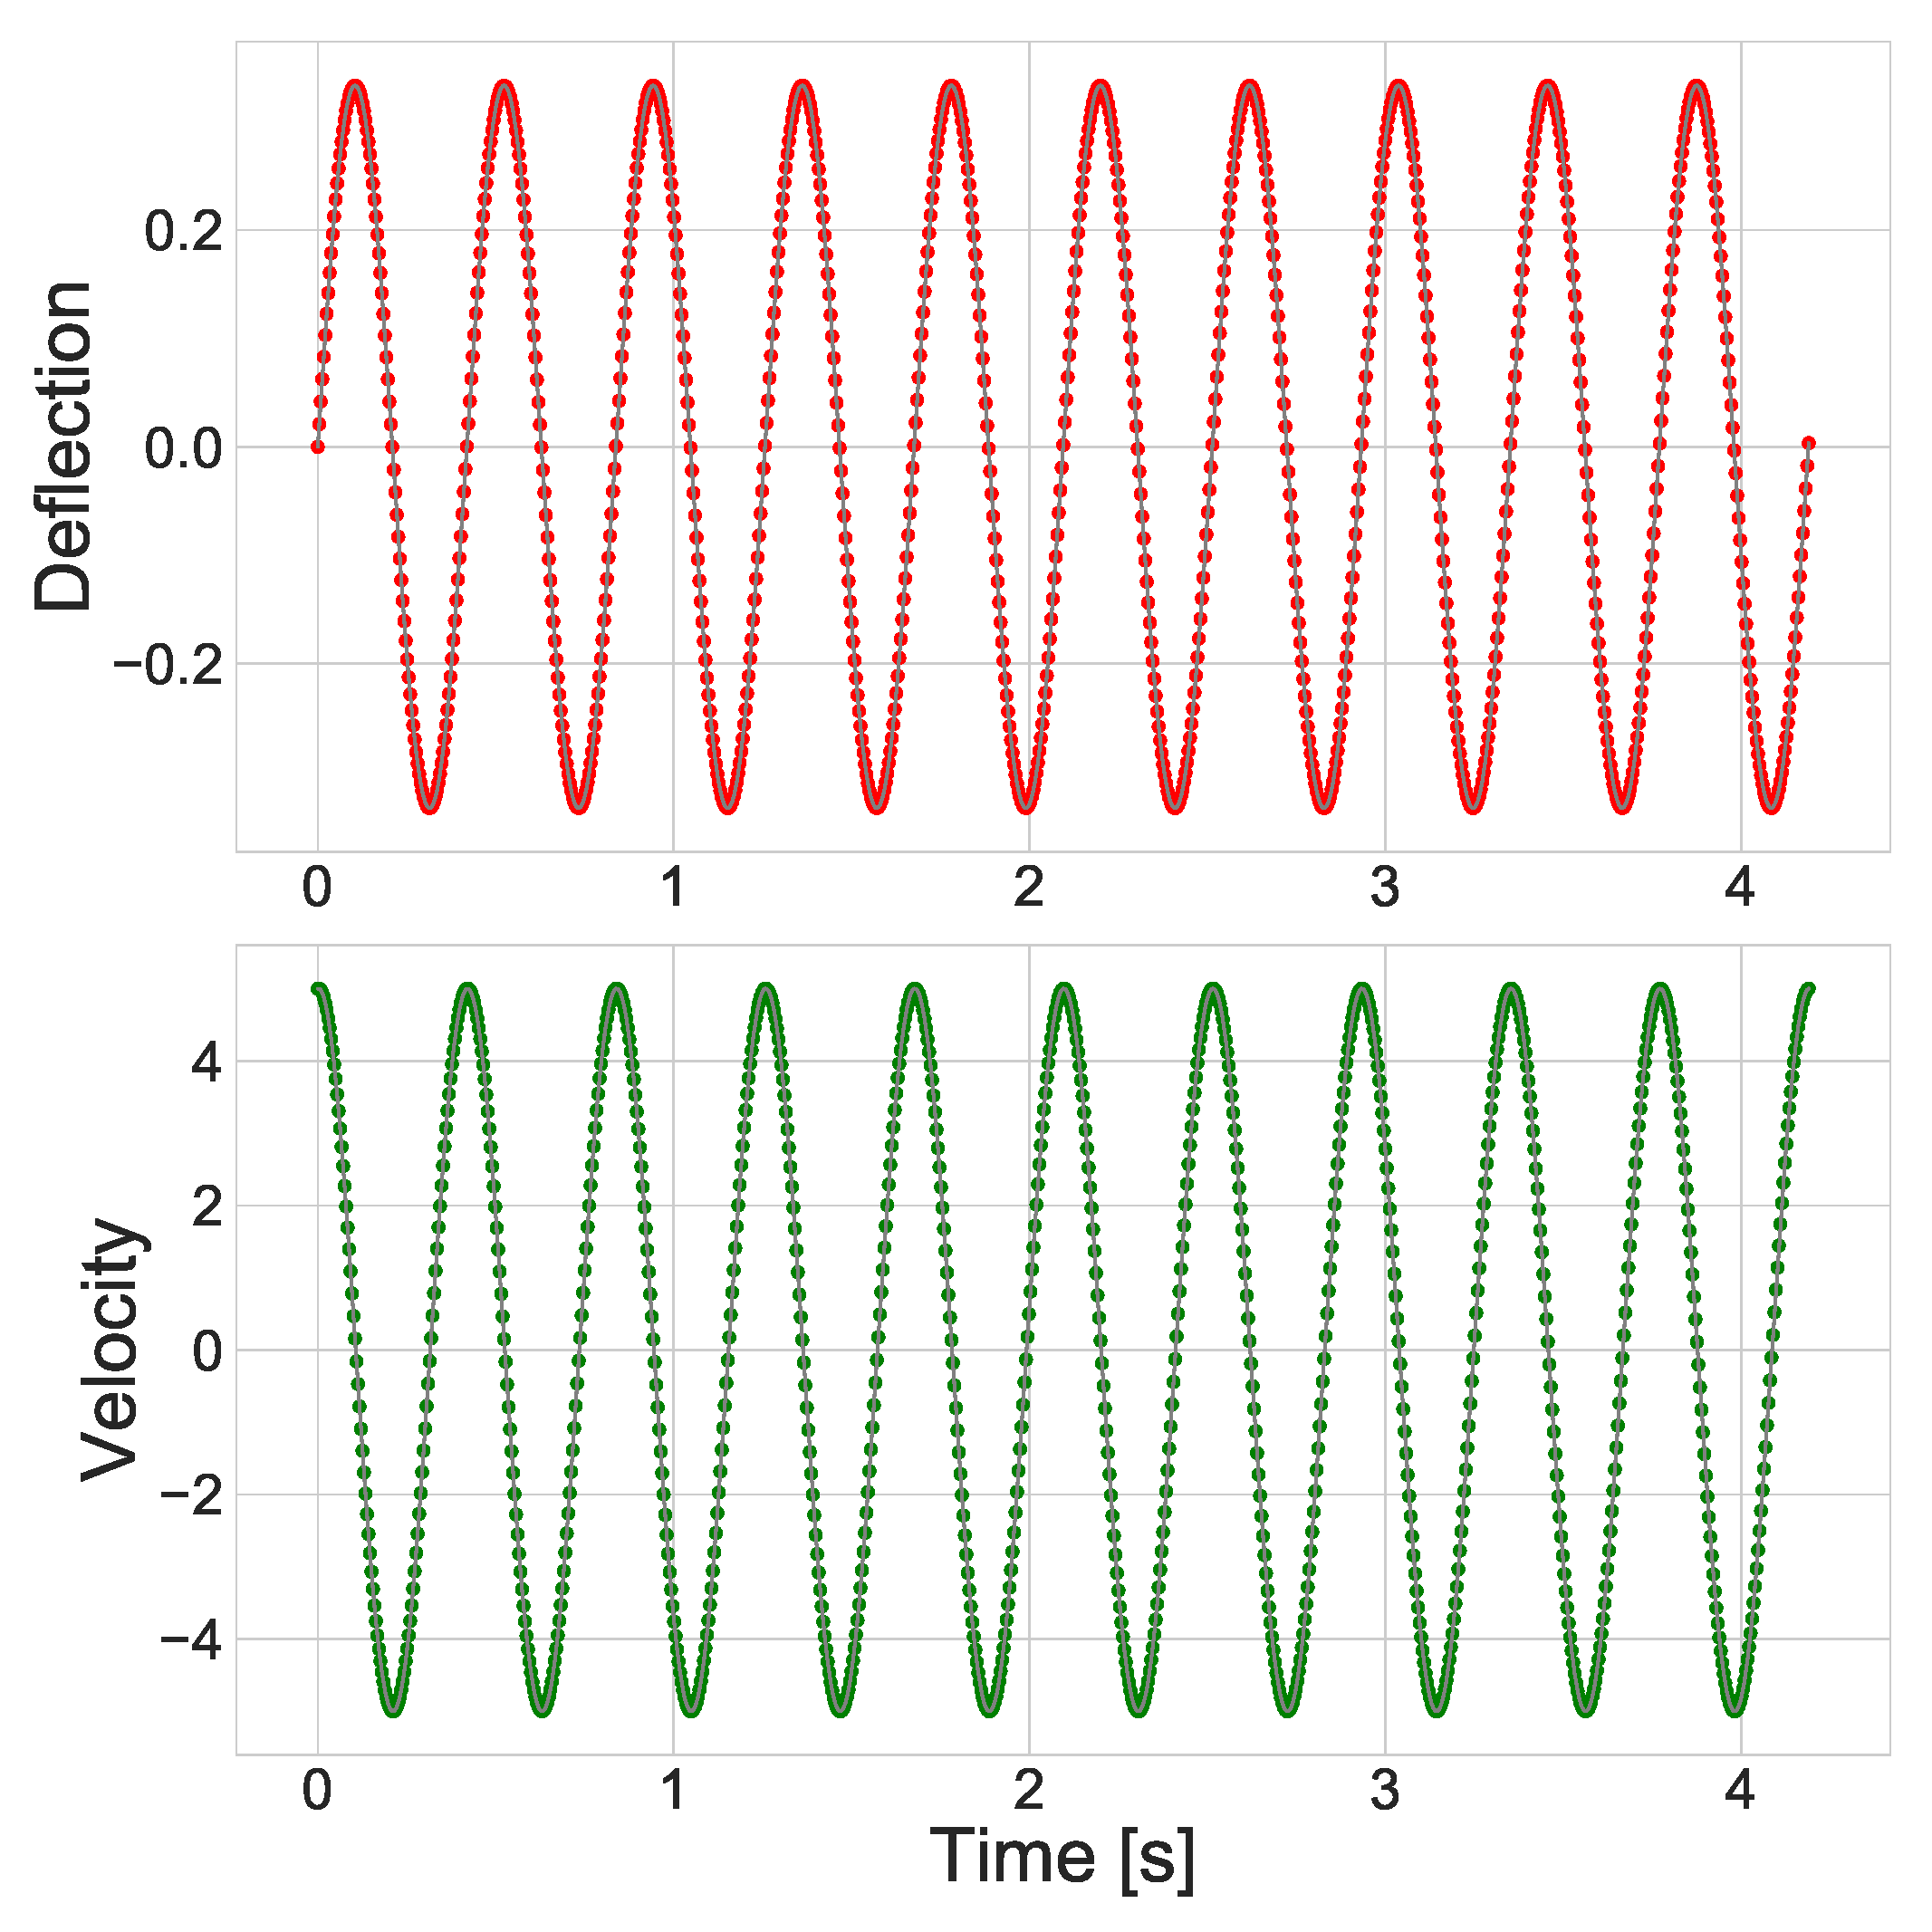
\includegraphics[width=.5\textwidth]{time_def_vel.eps}}
\captionof{figure}{\\Fent: Idő - Kitérés grafikon\\Alul: Idő- Sebesség grafikon}\label{fig1}
\hfill \break \hfill \break
A szimuláció során kapott adatok az első feladatnak megfelelően az \ref{fig1}. ábrán láthatóak. Ez a mélyebb megértés céljából egy sebesség-idő grafikonnal is ki lett bővítve. A kapott kép alapján az elméletből elvártakat kaptuk vissza. Az oszcillátor sebessége zéró kitérésnél a legnagyobb, maximális kitérésnél pont $0$, majd pedig előjelet vált.

\end{multicols}
\hrulefill